\documentclass[journal,twoside,web]{ieeecolor}
\usepackage{tmi}
\usepackage{cite}
\usepackage{amsmath,amssymb,amsfonts,physics}
\usepackage{algorithmic}
\usepackage{caption,subcaption}
\usepackage{siunitx}
\usepackage{graphicx}
\usepackage{textcomp}
\def\BibTeX{{\rm B\kern-.05em{\sc i\kern-.025em b}\kern-.08em
    T\kern-.1667em\lower.7ex\hbox{E}\kern-.125emX}}
\markboth{Advanced Computer Applications in Engineering}
{H. Dar: Computational Modelling of the Haemodynamics in Coiled and Uncoiled Cerebral Aneurysms}
\begin{document}
\title{Computational Modelling of the Haemodynamics in Coiled and Uncoiled Cerebral Aneurysms}
\author{Hasha Dar
    \thanks{Submitted on November 23, 2022.}
    \thanks{This work was completed as part of the assessment for the MECH0059 module, Mechanical Engineering Department, University College London. }
    \thanks{H. Dar is a fourth year undergraduate student on the MEng Mechanical Engineering Programme at University College London, London, WC1E 6BT (e-mail: hasha.dar.19@ucl.ac.uk). }}

\maketitle

\begin{abstract}
    This assignment investigates the use of computational fluid dynamics (CFD) to analyse the haemodynamics of cerebral aneurysms when treated via endovascular coil embolisation. I utilise a simplified model of a basilar bifurcated artery with a saccular aneurysm for this assignment. The area where coils are inserted are modelled as a porous medium and my results show a positive change in the haemodynamics of the artery. Specifically, the flow of blood and pressure is reduced to negligible in the saccular region of the aneurysm and the flow through the bifurcation is much improved. The results show that coil embolisation can be an effective treatment for a cerebral aneurysm - preventing it from growing or rupturing. This assignment simplifies the problem as to place emphasis on the ``CFD workflow,'' and to emulate the experience of an industrial engineer or researcher using CFD for a project.
\end{abstract}

\begin{IEEEkeywords}
    Cerebral aneurysms, endovascular coil embolisation, computational haemodynamics
\end{IEEEkeywords}

\section{Introduction}
\IEEEPARstart{C}{erebral} aneurysms are formed due to the deterioration of the normal arterial structure leading to a dilation or bulge in the vessel wall, typically called a sac. This will fill with blood and apply pressure to the surroundings areas; on nerves and adjacent brain tissue. The development of a saccular cerebral aneurysm (accounting for 90\% of cases) occurs in 1\% to 5\% of the general population - the majority of which are asymptomatic \cite{doi:10.1161/STROKEAHA.113.002390}. However, there is a risk that the aneurysm ruptures in approximately 2\% to 6\% of cases leading to significant intracranial bleeding \cite{doi:10.1161/01.STR.29.1.251}. In most cases, the diagnosis is a subarachnoid hemorrhage (SAH) and between 25\% to 50\% of SAH are fatal, with another 50\% resulting in disability \cite{intracranialAneurysms}.

Diagnosis of cerebral aneurysms is mainly done via angiography. The predominant imaging methods are intra-arterial digital subtraction angiography (IADSA), magnetic resonance angiography (MRA), and computed tomography angiography (CTA) \cite{doi:10.1177/1358863X18754693}. Detection of an aneurysm using these methods aim to inform a doctor of a course of treatment, depending on the size and location of the aneurysm. These imaging techniques allow for the treatment of cerebral aneurysms, with the prevailing method being endovascular coil embolisation. This treatment deposits a series of platinum coils into the cerebral aneurysm through the use of a guided microcatheter \cite{Pouratian572}. The result of this is a reduction of blood flow and thrombosis within the aneurysm, preventing a rupture and SAH. This is an effective treatment as the mortality of treated patients is vastly reduced: 1-year mortality rate of 3.1\% \cite{1231234}.

Computational fluid dynamics can be used to model the haemodynamics of cerebral aneurysms. Indeed, the understanding of the flow characteristics is important for the effective of treatment of saccular aneurysms.
\section{Methods}
\subsection{Overview}
In this section, I will introduce the methods used in modelling the haemodynamics of a basilar bifurcated artery with a saccular cerebral aneurysm. Specifically, an investigation into the flow before and after coil embolisation is outlined in this paper. This paper also investigates modelling of the working fluid (blood) as a Newtonian and non-Newtonian fluid. The effects of coil embolisation are characterised through the setting of the saccular region of the aneurysm as a porous medium. This has been performed in previous work such as Kakalis \textit{et al} \cite{30180980813}.

Hence, we shall be looking at four cases within this paper. These shall be referred to as `Case x' in this paper. The cases are:
\begin{enumerate}
    \item An uncoiled Newtonian case, with physiological flow (the base case)
    \item A coiled Newtonian case, with physiological flow
    \item An uncoiled non-Newtonian case, with physiological flow
    \item A coiled non-Newtonian case, with physiological flow
\end{enumerate}

The blood flow model is discussed in \ref{flows}. The geometry of the vasculature and its construction is outlined in section \ref{geom}. Meshing and justification of mesh size and type is shown in section \ref{mesh}. Specifics regarding the solver setup are shown in section \ref{solverSetup}.
\subsection{Modelling of Blood Flow}\label{flows}
Due to the scope and aims of this assignment, certain assumptions and simplifications have been made. A steady flow scheme was chosen to model the haemodynamics. Pulsatile flow, although a better representation of blood flow along the cardiac cycle, would represent a further complexity. Steady flow modelling is sufficient to explore the relative changes of blood flow before and after coil embolisation. Another assumption made in the interest of simplification are rigid walls - blood vessels are elastic - where a pulsatile flow would show changes in the haemodynamics. There is little relevance of the transient effects (on the cardiac cycle scale) to the scope of this project. Hence, the use of a substantially less computationally intensive steady flow scheme is favourable and justified.
\subsubsection{Newtonian fluid model}
The Newtonian fluid model describes that a fluid has a linear viscous flow behaviour - the shear rate is proportional to the shear stress (at constant temperature and pressure). Another assumption is that the flow is incompressible. Equation \eqref{Eq1} describes this mathematical relationship.
\begin{equation}\label{Eq1}
    \tau = \mu_d \frac{\textrm{d}u}{\textrm{d}y}
\end{equation}
where $\tau$ is the shear stress in \si{\pascal}, $\mu_d$ is the dynamic viscosity in \si{\pascal\second} and $\frac{\textrm{d}u}{\textrm{d}y}$ is the shear rate in \si{\per\second}. In the cases using the Newtonian fluid model, a constant density of $\rho = \SI{1060}{kg\per\meter\cubed}$ and a constant dynamic viscosity of $\mu = \SI{3.57e-3}{kg\per\meter\second}$ were chosen.

The flow can be characterised using the Navier-Stokes equations and are shown in \eqref{Eq2} and \eqref{Eq3}.
\begin{equation}\label{Eq2}
    \frac{\partial \vb{u}}{\partial t} + \left(\vb{u\cdot \nabla}\right)\vb{u} = - \vb{\nabla}\left(\frac{p}{\rho}\right) + \nu \vb{\nabla^2 u}
\end{equation}
\begin{equation}\label{Eq3}
    \nabla \cdot \vb{u} = 0
\end{equation}
where $\vb{u}$ is the flow velocity, $t$ is time, $\nabla$ is the divergence, $p$ is the pressure, $\rho$ is the density and $\nu = \frac{\mu}{\rho_0}$ is the kinematic viscosity.
\subsubsection{Non-Newtonian fluid model}
A non-Newtonian fluid is characterised by a viscosity that varies with strain rate. These fluids may not be characterised as having a well-defined viscosity. Hence, other fluid parameters may be utilised to define the fluid, such as oscillatory shear or extensional flow. A key characteristic of our working fluid (blood) is it's shear thinning behaviour i.e. the viscosity of blood reduces as the diameter of the vessel reduces and shear stress reduces. This attribute allows blood to reach even the smallest of blood vessels and capillaries. This is known as the Fahraeus-Lindqvist effect and the behaviour is displayed until the blood vessel diameter reaches to that of individual red blood cells, where the viscosity increases.

One non-Newtonian model for blood is the Blood Power Law and is shown in \eqref{Eq4}, \eqref{Eq5} and \eqref{Eq6}.
\begin{equation}\label{Eq4}
    \mu = \delta \left|\gamma \right|^{n-1}
\end{equation}
\begin{equation}\label{Eq5}
    \delta \left(\gamma \right)= \mu_{\infty} + \delta \mu \exp\left[-\left(1 + \left(\frac{\left|\gamma\right|}{a}\right)\right)\exp\left(\frac{-b}{\left|\gamma\right|}\right)\right]
\end{equation}
\begin{equation}\label{Eq6}
    n\left(\gamma\right) = n_{\infty} - \delta n \exp\left[-\left(1 + \left(\frac{\left|\gamma\right|}{c}\right)\right)\exp\left(\frac{-d}{\left|\gamma\right|}\right)\right]
\end{equation}
where $\gamma$ is the local calculated shear stress, $\delta$ is the consistency constant, $\mu_{\infty} = 0.035$ is the limiting (Newtonian) viscosity (default value) and $\delta \mu = 0.25$ is the change in viscosity (default value). $a = 50$, $b = 3$, $c = 50$, $d = 4$ are all constants with default values preset by CFD-ACE+.
\subsection{Geometry to Model Cerebral Aneurysm}\label{geom}
\begin{figure}[!t]
    \centerline{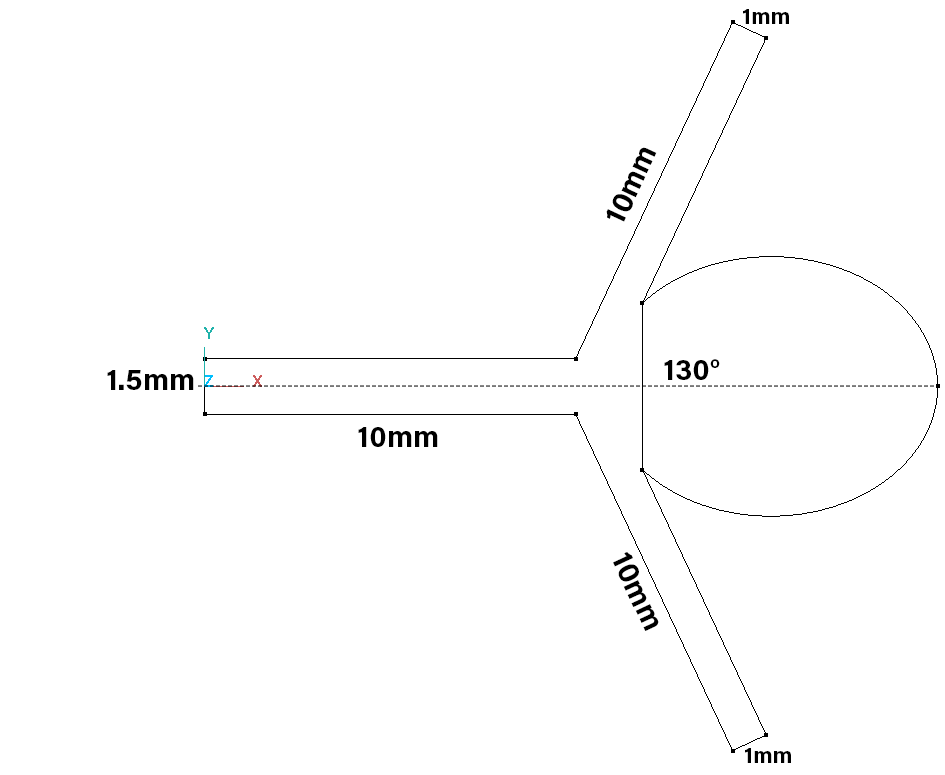
\includegraphics[width=\columnwidth]{img/fig1.png}}
    \caption{2D geometry of basilar bifurcated artery with saccular aneurysm.}
    \label{fig1}
\end{figure}
In Figure \ref{fig1}, we can see the simplified geometry of a basilar bifurcated artery with saccular aneurysm. Here, the vasculature is symmetric to aid in the simplification of the system. Another key simplification is the choice to utilise a 2D geometry. The aim of this paper is to investigate the CFD workflow; 3D modelling the vasculature is a complex task and was not performed.

The dimensions of the main vasculature are \SI{1.5}{mm} by \SI{10}{mm} and lead into two separate branches with a reduced cross section of \SI{1}{mm}. The sac is modelled as a ellipse with a major radius of \SI{4.5}{mm} and minor radius \SI{3.5}{mm}. CFD-GEOM was used to model the geometry.
\subsection{Generation of Mesh}\label{mesh}
The geometry was meshed using an unstructured triangular mesh. This is justified as this mesh structure can reproduce the curvature of the sac to an acceptable level. Modelling the vasculature structure with a structured mesh may prove ideal for the regular sections of the geometry but would pose problems within the saccular section - arguably the most important section of interest within this geometry. An ideal mesh would have been constructed with due consideration for the differences in geometry for different parts of the vasculature. Another advantage of a triangular mesh is the ease in which our mesh density can be changed. This is important as validation of the mesh requires performing a variety of simulations at varying mesh densities to demonstrate grid independence.

\begin{figure}[!t]
    \centerline{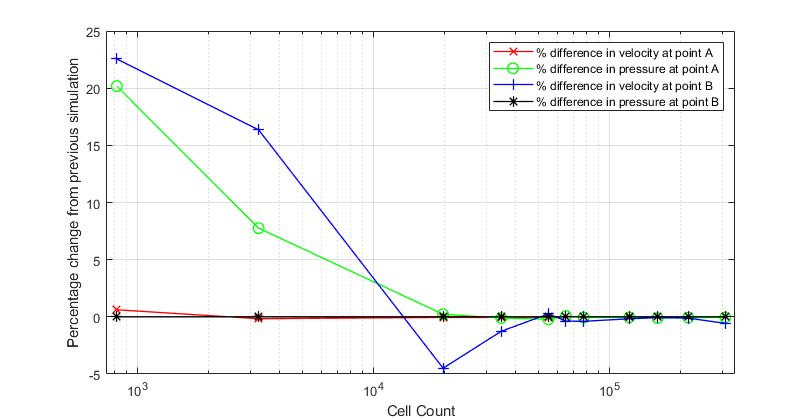
\includegraphics[width=\columnwidth]{img/fig2.png}}
    \caption{Graph to show percentage difference of velocity and pressure at two different points within the mesh against number of cells in mesh at two points: A \& B.}
    \label{fig2}
\end{figure}

Grid independence simulations were performed using Case 1 - the base case. In Figure \ref{fig2}, we can see that data was collected from 12 simulations with varying mesh densities. Cell counts ranging from below \SI{10e3} to over \SI{10e5} were used. To test whether grid independence had been achieved, two points were indexed within the mesh:
\begin{enumerate}
    \item Point A - (\SI{0.1}{mm}, \SI{0}{mm})
    \item Point B - (\SI{2}{mm}, \SI{0}{mm})
\end{enumerate}
where Point A represents an index point close to the inlet of main vasculature and Point B represents an index point along the main vasculature. The significance of choosing points close to the inlet and within the main vasculature is to index a point where the flow is predictable. In the saccular region, the flow may rotate clockwise or anti-clockwise. This discrepancy can be attributed to the fact that in each simulation, the structure of the mesh can cause the flow to deviate slightly early on. These small deviations will manifest throughout the rest of the simulation - one such manifestation is the direction of the vortex. The percentage difference was calculated using the value from the previous simulation (simulations were conducted from small cell count to large cell count).

From Figure \ref{fig2}, we can see a clear convergence of the velocity and pressure at both points as the cell count approaches 50,000. The percentage difference in the aforementioned parameters is below 0.1\% when the mesh size is increased further. Hence, a cell count of 65302 (representing a maximum cell size of 0.055) was utilised for all cases. This mesh size also commands a reasonable computational time of approximately 22 minutes.

\subsection{Modelling of Coil Embolisation via Porous Media}
Direct modelling of the coils within the aneurysm is a complex task. Previous work such as Umeda \textit{et al} and Li \textit{et al} have shown that modelling the coils as a porous medium is an effective substitute \cite{10.1371/journal.pone.0190222}, \cite{1231512}. The geometry of the porous region can be seen in Figure \ref{fig2}, as the elliptical sac. Here the boundary between the porous region and the arterial vasculature is modelled as a straight line. An isotropic resistance model was used within CFD-ACE+ with the following parameters:
\begin{itemize}
    \item Linear resistance porosity: 0.8
    \item Linear resistance permeability: \SI{1e-8}{m^2}
\end{itemize}

\subsection{Solver Setup}\label{solverSetup}
\subsubsection{Boundary Conditions}
The inlet wall was configured with a fixed velocity condition. The inlet x-direction velocity of \SI{0.27}{\meter\per\second} and temperature \SI{310}{\kelvin} - to represent the incoming blood flow - were chosen. The outlet walls were configured with a fixed pressure condition and a backflow temperature of \SI{310}{\kelvin}. These values were fixed as a constant body temperature can be assumed.
\subsubsection{Initial Conditions}
An initial temperature of \SI{310}{\kelvin} was chosen as a constant body temperature can be assumed. Cases 3 and 4 were setup with a previous solution initial condition; cases 1 and 2 respectively.
\subsubsection{Solver Conditions}
Some general information regarding the solver settings are listed below:
\begin{itemize}
    \item Maximum iterations: 4000 (adjusted to higher values to reach convergence)
    \item Spatial differencing method for velocity: central method with 0.1 blending factor
    \item Solvers
          \begin{itemize}
              \item Velocity: algebraic multigrid solver with 5 sweeps and 0.01 criterion
              \item Pressure correction: algebraic multigrid solver with 10 sweeps and 0.1 criterion
          \end{itemize}
\end{itemize}
\section{Results and Discussion}
Figures \ref{geom15V}, \ref{geom17V}, \ref{geom16V}, \ref{geom18V} show the velocity magnitudes of the flow for each case. In Case 1 and 3, we see that the flow is distributed unequally between the two outlet vasculature. This unequal flow can prove problematic as this can lead to ischaemic problems within other parts of the cerebral vasculature. In Case 2 and 4, we see an equal distribution of the fluid between the two outlet vasculature. We can see a clear stagnation in fluid velocity as the fluid approaches the boundary of the aneurysm, and the flow is redirected to the vasculature equally.

Comparing the uncoiled cases to the coiled cases, we see that the flow is no longer entering the aneurysm sac and the fluid velocity is reduced to below \SI{0.05}{m\per \second}. This is a positive change in the haemodynamics as stagnation of the blood flow within the saccular region would promote thrombosis and prevent further growth of the sac.

Comparing the Newtonian cases with the non-Newtonian cases, we find that there is a small percentage difference between the two simulations. Indexing points close to the boundary of the aneurysm yielded a percentage difference of 0.06\% in velocity magnitudes between the two simulations (index point: (0.009,0)). This shows that modelling the flow using the Blood Power Law yields no significant benefit over a Newtonian model for the additional computational time and complexity.

\begin{figure}[!t]
    \centerline{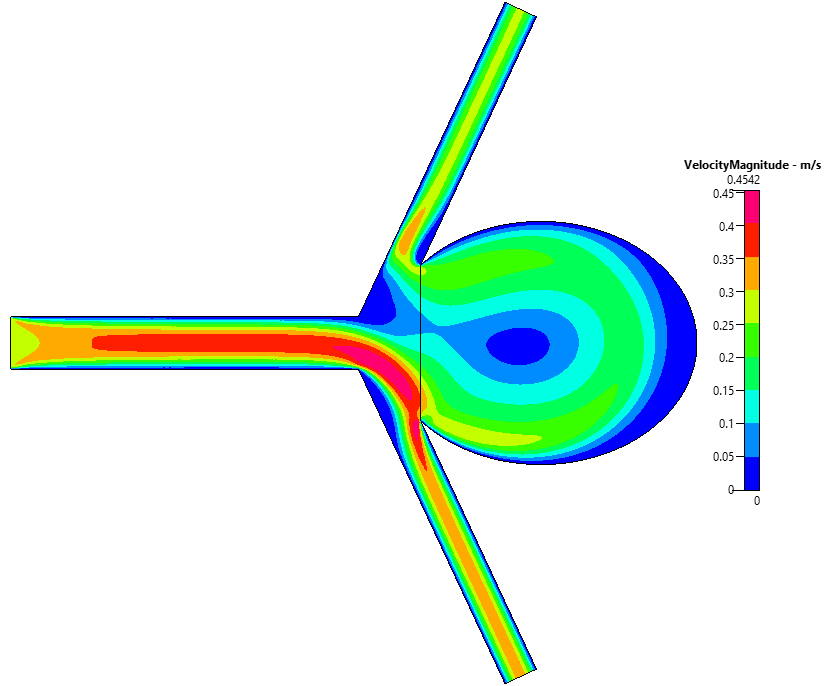
\includegraphics[width=\columnwidth]{img/geom15Velocity.png}}
    \caption{Plot of velocity contours for Case 1 - Newtonian Uncoiled.}
    \label{geom15V}
\end{figure}
\begin{figure}[!t]
    \centerline{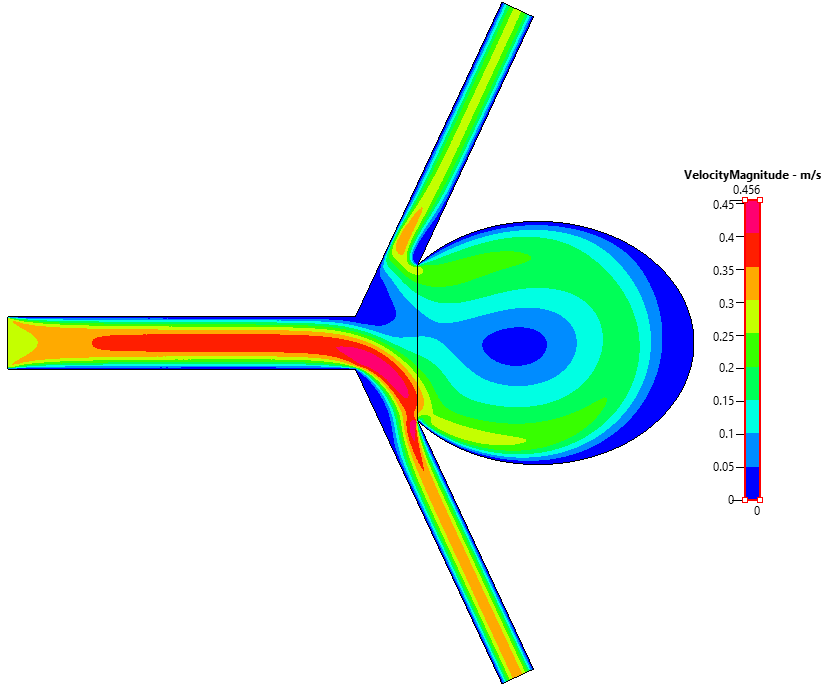
\includegraphics[width=\columnwidth]{img/geom17Velocity.png}}
    \caption{Plot of velocity contours for Case 2 - Newtonian Coiled.}
    \label{geom17V}
\end{figure}
\begin{figure}[!t]
    \centerline{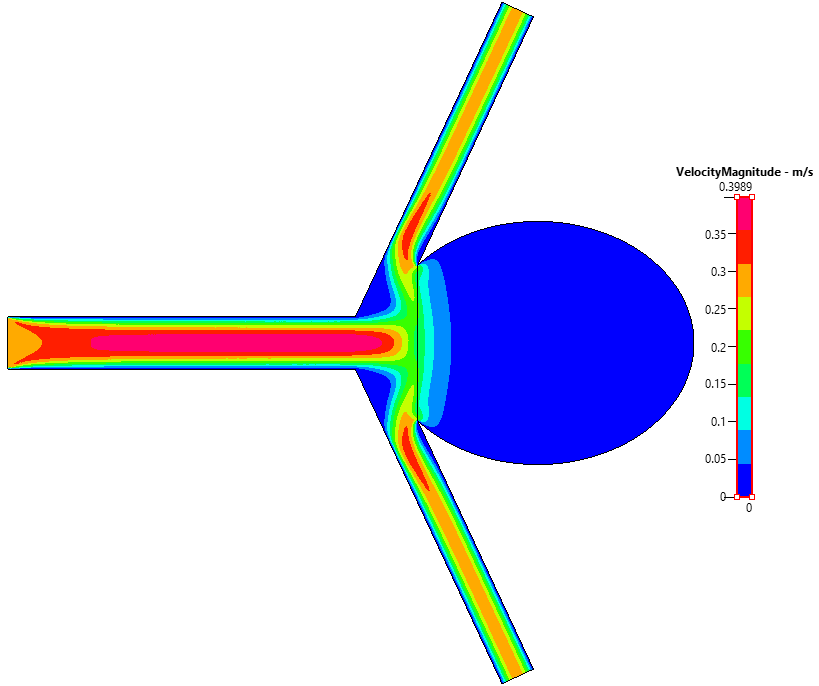
\includegraphics[width=\columnwidth]{img/geom16Velocity.png}}
    \caption{Plot of velocity contours for Case 3 - non-Newtonian Uncoiled.}
    \label{geom16V}
\end{figure}
\begin{figure}[!t]
    \centerline{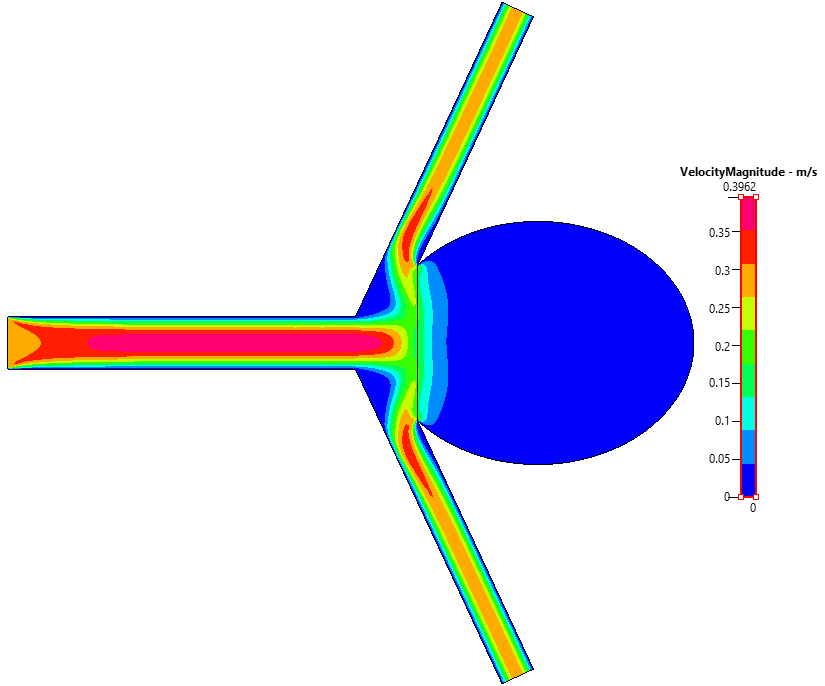
\includegraphics[width=\columnwidth]{img/geom18Velocity.png}}
    \caption{Plot of velocity contours for Case 4 - non-Newtonian Coiled.}
    \label{geom18V}
\end{figure}

Figures \ref{geom17P}, \ref{geom18P} show the pressure distribution in Case 3 and 4. We see that pressure differential in case 3 is uneven and there is a little variation in the pressure from the latter portion of the inlet vasculature to the saccular region, allowing blood to flow through without losing much energy. We can also see the uneven distribution of pressure between the two outlet vasculature. Comparatively, we see that in the coiled case, the saccular region transitions into a higher pressure region. This serves to stagnate the blood flow and allow any entering blood to thrombose. This would further increase the resistance to flow within the saccular region. We can see that there is a point of very high pressure along the symmetry line, however this would be an artefact of our symmetrical and simplified geometry. In an anatomically correct model, we may see a much more complicated pressure differential on the boundary between the saccular region and the vasculature. Another interesting development is the higher average pressures within the saccular region. This trade-off is favourable to prevent the uneven flow of blood within the vasculature.

\begin{figure}[!t]
    \centerline{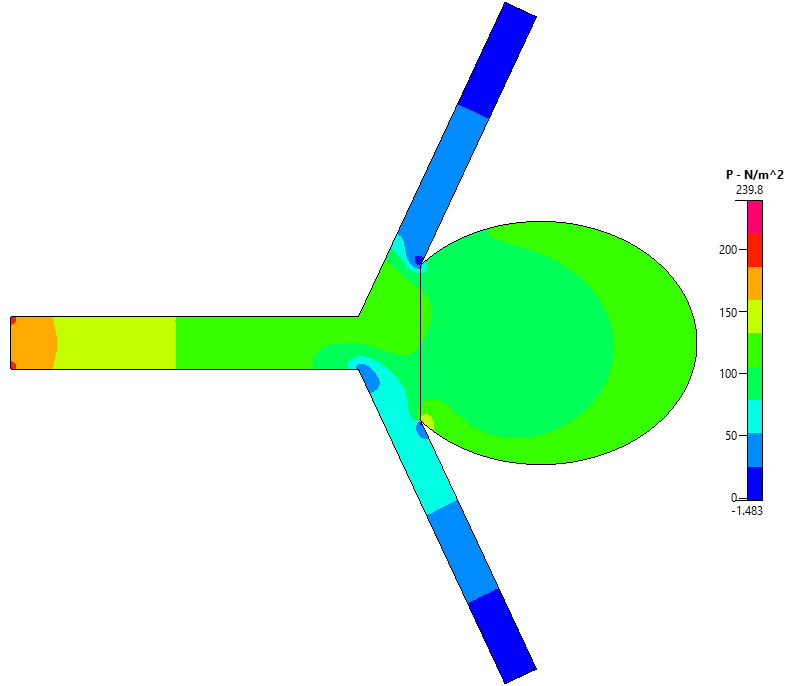
\includegraphics[width=\columnwidth]{img/geom17Pressure.png}}
    \caption{Plot of pressure contours for Case 3 - non-Newtonian Uncoiled.}
    \label{geom17P}
\end{figure}
\begin{figure}[!t]
    \centerline{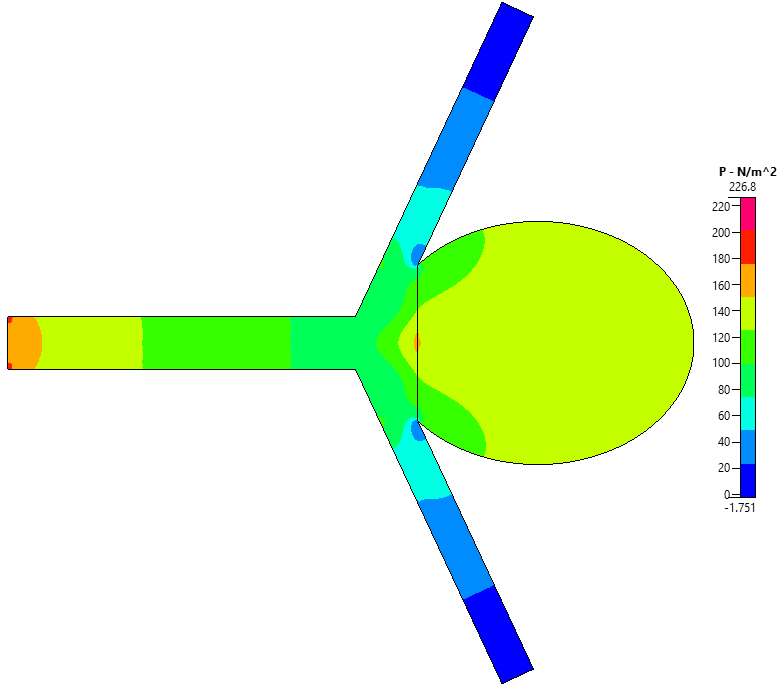
\includegraphics[width=\columnwidth]{img/geom18Pressure.png}}
    \caption{Plot of pressure contours for Case 4 - non-Newtonian Coiled.}
    \label{geom18P}
\end{figure}

Figure \ref{geom17S}, \ref{geom18S} show the strain rate plots for Case 3 and 4. Here, we see that the maximum strain rate occurs at the inlet wall. This can be considered an artefact of the simulation as in reality, this vasculature would extend much farther. In the region of interest, we see that the strain rate is localised at the boundary between the sac and the outlet wall. In the uncoiled case, this value is approximately \SI{7700}{\per\second}. A significant reduction in the localised strain rate is seen in the coiled simulation, dropping by 66\% to approximately \SI{2600}{\per\second}. In Figure \ref{strain1}, we can see that the strain rate in the uncoiled case at the end of saccular region increases. The coiling process reduces this to negligible. However, we do see an increase in the strain rate in the region of bifurcation. This trade-off is acceptable in order to reduce the risk of growth and subsequent rupture of the saccular region.

\begin{figure}[!t]
    \centerline{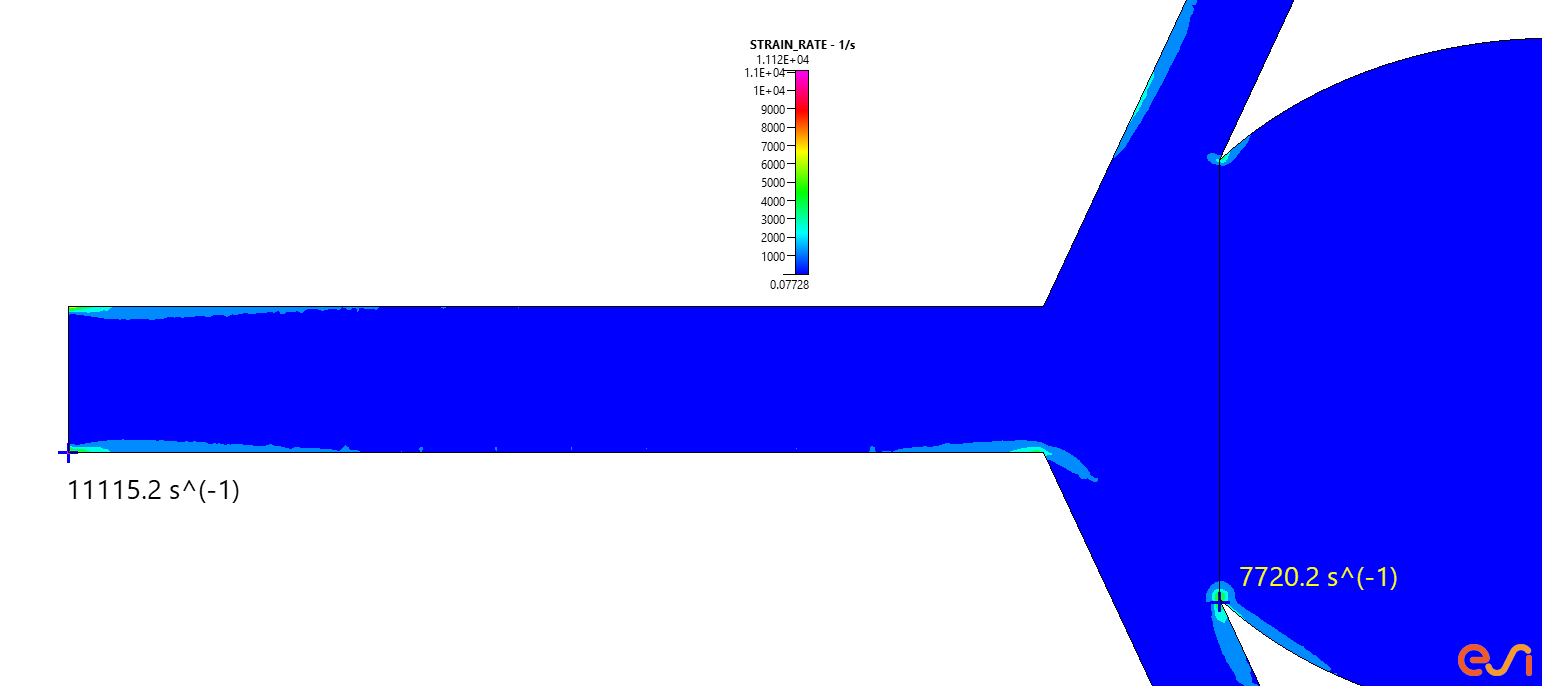
\includegraphics[width=\columnwidth]{img/geom17Strain.png}}
    \caption{Plot of velocity contours for Case 3 - non-Newtonian Uncoiled.}
    \label{geom17S}
\end{figure}
\begin{figure}[!t]
    \centerline{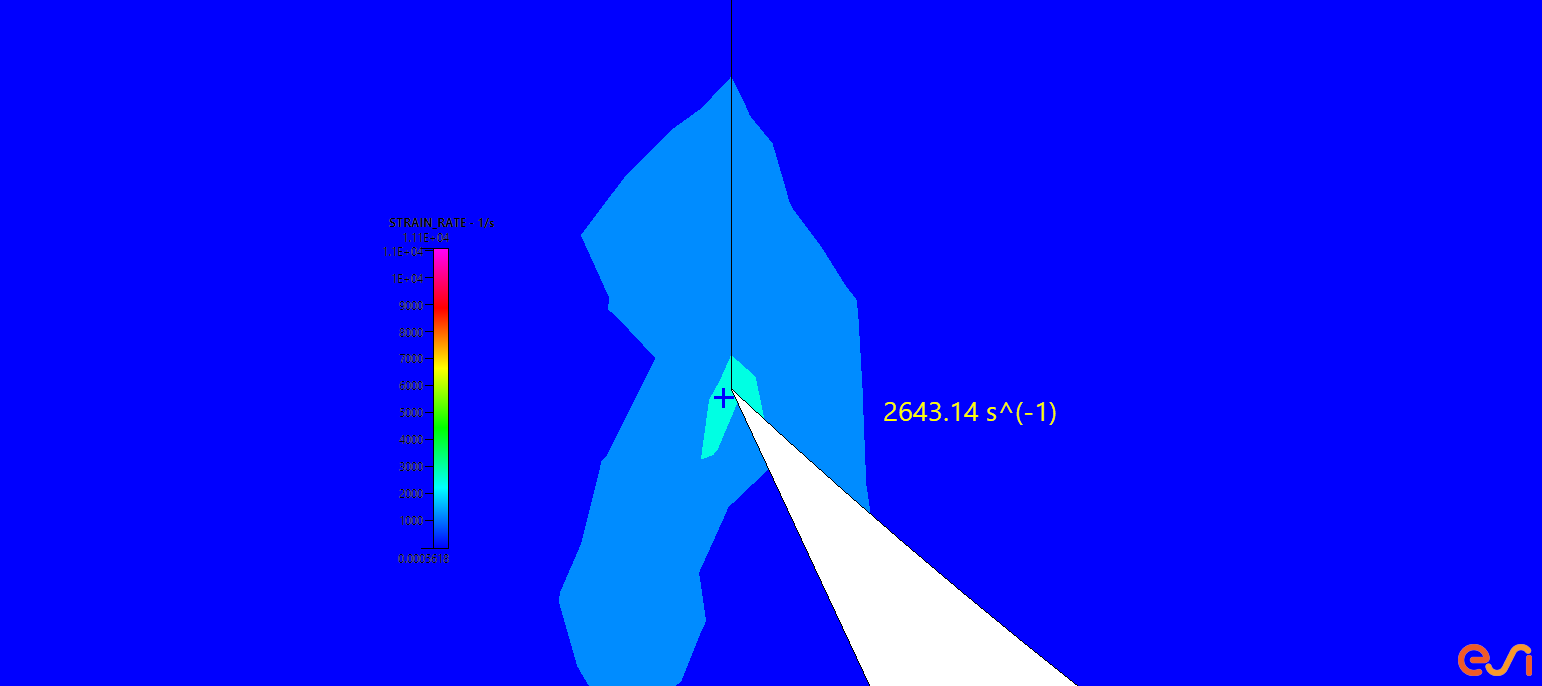
\includegraphics[width=\columnwidth]{img/geom18Strain.png}}
    \caption{Plot of velocity contours for Case 4 - non-Newtonian Coiled.}
    \label{geom18S}
\end{figure}
\begin{figure}[!t]
    \centerline{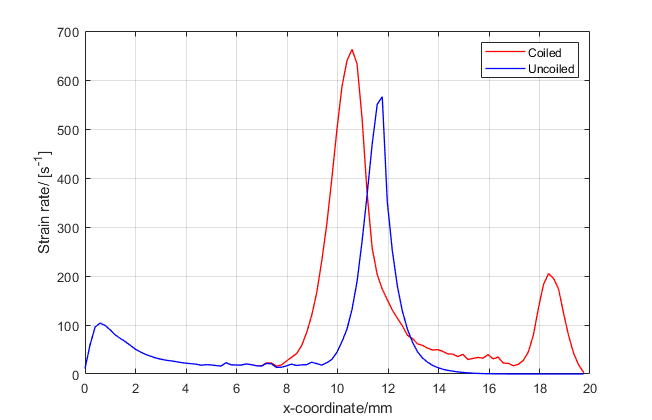
\includegraphics[width=\columnwidth]{img/fig4.png}}
    \caption{Plot of strain rate along axis of symmetry for Case 3 and 4.}
    \label{strain1}
\end{figure}
\section{Conclusion}
This paper outlines some of the features of a CFD workflow. The results shown here indicate that coil embolisation is effective in positively altering the haemodynamics of a saccular aneurysm located near a basilar bifurcated vasculature. Further work may include verification of the model via experimentation or to model an aneurysm derived from angiography in 3D.
\section*{Acknowledgment}
The ESI Group (Paris, France), developers of the CFD-ACE+ multiphysics software platform, are kindly acknowledged for allowing the use of the software for this assignment.
\bibliographystyle{vancouver}
\bibliography{refs}
\end{document}